% FILENAME: paper/section-Appendix.tex

\appendix

\section{Formal Verification Methodology and \texttt{Litlib}}
% TODO for Author: Address the epistemology of formal verification. Explain that while the core topological mechanics of CGD are formalized from scratch, we use a secure library of axiomatic signatures (`Litlib`) to import established 20th-century differential geometry theorems (Geroch-Jang, Capovilla-Dell-Jacobson, etc.). Explain how the Lean 4 class system strictly enforces the boundaries of these unformalized assumptions to guarantee mathematical transparency.

\section{Phenomenological Implications: The Proton Radius}
% TODO for Author: Explain how the 1D flux tube / instanton geometry maps to empirical scattering data. Discuss the implications of the plot.

\begin{figure}[htbp]
    \centering
    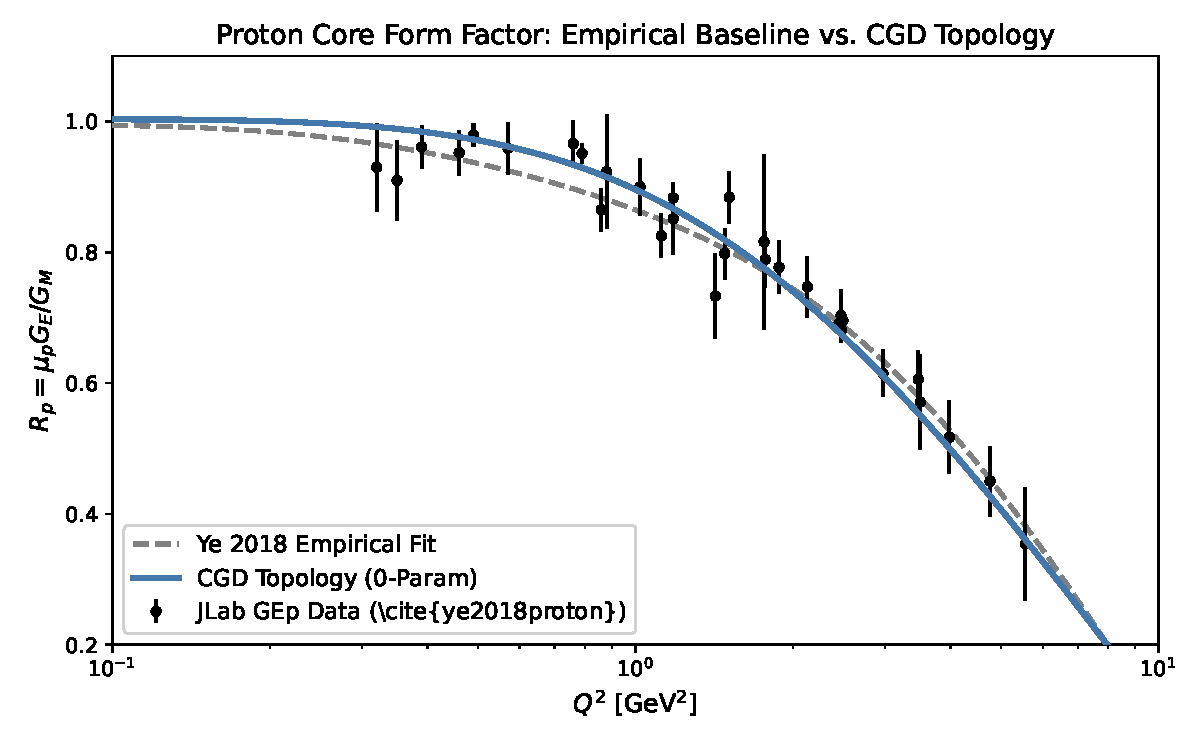
\includegraphics[width=\linewidth]{cgd_appendix_plot.pdf}
    \caption{\todo{Explain the proton radius plot thoroughly}}
    \label{fig:proton_radius}
\end{figure}
